% =========================================================================
% Despedida de Pedro (Piter T), última ayudantía 2026
% Caja de cierre del libro con pato grande. Se oculta con \mostrarTipsfalse.
% El coordinador la cablea (% =========================================================================
% Despedida de Pedro (Piter T), última ayudantía 2026
% Caja de cierre del libro con pato grande. Se oculta con \mostrarTipsfalse.
% El coordinador la cablea (% =========================================================================
% Despedida de Pedro (Piter T), última ayudantía 2026
% Caja de cierre del libro con pato grande. Se oculta con \mostrarTipsfalse.
% El coordinador la cablea (% =========================================================================
% Despedida de Pedro (Piter T), última ayudantía 2026
% Caja de cierre del libro con pato grande. Se oculta con \mostrarTipsfalse.
% El coordinador la cablea (\input{Contenidos/Despedida}) donde corresponda.
% =========================================================================
\ifmostrarTips
\clearpage
\begin{center}
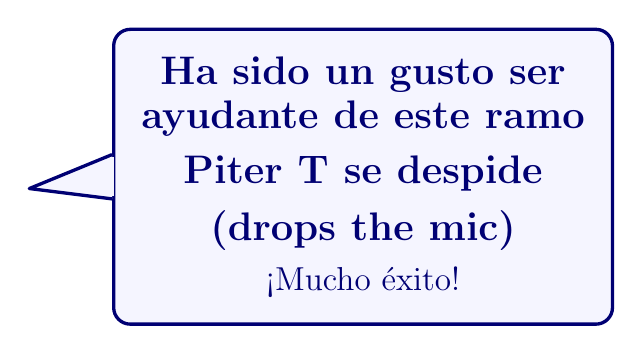
\begin{tikzpicture}
  % Pato grande y formal
  \begin{scope}[scale=1.6]
    \duck[body=gray!20, jacket=blue!45!black, tie=red!60!black,
          graduate=blue!45!black, tassel=red!60!black,
          book={}, bookcolour=red!45!black]
  \end{scope}
  % Globo de diálogo (sin librerías extra)
  \node[draw=blue!45!black, fill=blue!4, rounded corners=6pt, very thick,
        text=blue!45!black, align=center, inner sep=10pt, anchor=west] (despedida) at (3.6,2.9)
        {{\Large\bfseries Ha sido un gusto ser}\\[2pt]
         {\Large\bfseries ayudante de este ramo}\\[6pt]
         {\Large\bfseries Piter T se despide }\\[6pt]
         {\Large\bfseries (drops the mic)}\\[6pt]
         {\large ¡Mucho éxito!}};
  \filldraw[draw=blue!45!black, fill=blue!4, very thick, line join=round]
    ([yshift=8pt]despedida.west) -- (2.55,2.75) -- ([yshift=-8pt]despedida.west);
  \fill[blue!4] ([xshift=-0.8pt,yshift=7pt]despedida.west)
    rectangle ([xshift=0.8pt,yshift=-7pt]despedida.west);
\end{tikzpicture}
\end{center}
\fi
) donde corresponda.
% =========================================================================
\ifmostrarTips
\clearpage
\begin{center}
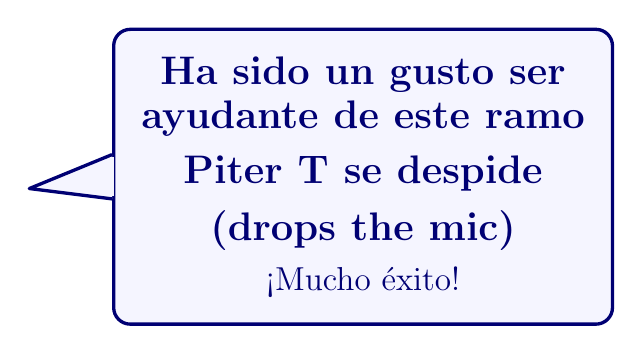
\begin{tikzpicture}
  % Pato grande y formal
  \begin{scope}[scale=1.6]
    \duck[body=gray!20, jacket=blue!45!black, tie=red!60!black,
          graduate=blue!45!black, tassel=red!60!black,
          book={}, bookcolour=red!45!black]
  \end{scope}
  % Globo de diálogo (sin librerías extra)
  \node[draw=blue!45!black, fill=blue!4, rounded corners=6pt, very thick,
        text=blue!45!black, align=center, inner sep=10pt, anchor=west] (despedida) at (3.6,2.9)
        {{\Large\bfseries Ha sido un gusto ser}\\[2pt]
         {\Large\bfseries ayudante de este ramo}\\[6pt]
         {\Large\bfseries Piter T se despide }\\[6pt]
         {\Large\bfseries (drops the mic)}\\[6pt]
         {\large ¡Mucho éxito!}};
  \filldraw[draw=blue!45!black, fill=blue!4, very thick, line join=round]
    ([yshift=8pt]despedida.west) -- (2.55,2.75) -- ([yshift=-8pt]despedida.west);
  \fill[blue!4] ([xshift=-0.8pt,yshift=7pt]despedida.west)
    rectangle ([xshift=0.8pt,yshift=-7pt]despedida.west);
\end{tikzpicture}
\end{center}
\fi
) donde corresponda.
% =========================================================================
\ifmostrarTips
\clearpage
\begin{center}
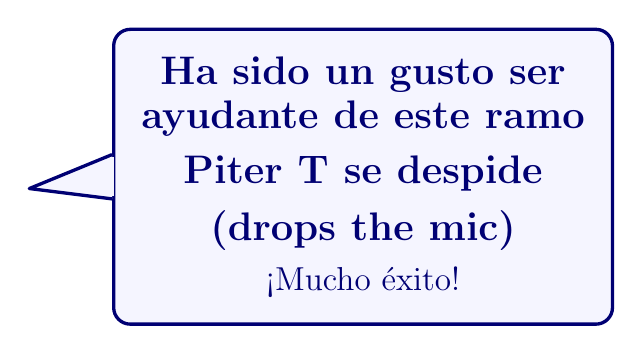
\begin{tikzpicture}
  % Pato grande y formal
  \begin{scope}[scale=1.6]
    \duck[body=gray!20, jacket=blue!45!black, tie=red!60!black,
          graduate=blue!45!black, tassel=red!60!black,
          book={}, bookcolour=red!45!black]
  \end{scope}
  % Globo de diálogo (sin librerías extra)
  \node[draw=blue!45!black, fill=blue!4, rounded corners=6pt, very thick,
        text=blue!45!black, align=center, inner sep=10pt, anchor=west] (despedida) at (3.6,2.9)
        {{\Large\bfseries Ha sido un gusto ser}\\[2pt]
         {\Large\bfseries ayudante de este ramo}\\[6pt]
         {\Large\bfseries Piter T se despide }\\[6pt]
         {\Large\bfseries (drops the mic)}\\[6pt]
         {\large ¡Mucho éxito!}};
  \filldraw[draw=blue!45!black, fill=blue!4, very thick, line join=round]
    ([yshift=8pt]despedida.west) -- (2.55,2.75) -- ([yshift=-8pt]despedida.west);
  \fill[blue!4] ([xshift=-0.8pt,yshift=7pt]despedida.west)
    rectangle ([xshift=0.8pt,yshift=-7pt]despedida.west);
\end{tikzpicture}
\end{center}
\fi
) donde corresponda.
% =========================================================================
\ifmostrarTips
\clearpage
\begin{center}
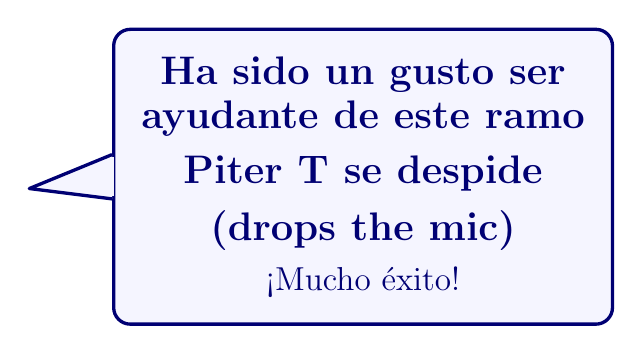
\begin{tikzpicture}
  % Pato grande y formal
  \begin{scope}[scale=1.6]
    \duck[body=gray!20, jacket=blue!45!black, tie=red!60!black,
          graduate=blue!45!black, tassel=red!60!black,
          book={}, bookcolour=red!45!black]
  \end{scope}
  % Globo de diálogo (sin librerías extra)
  \node[draw=blue!45!black, fill=blue!4, rounded corners=6pt, very thick,
        text=blue!45!black, align=center, inner sep=10pt, anchor=west] (despedida) at (3.6,2.9)
        {{\Large\bfseries Ha sido un gusto ser}\\[2pt]
         {\Large\bfseries ayudante de este ramo}\\[6pt]
         {\Large\bfseries Piter T se despide }\\[6pt]
         {\Large\bfseries (drops the mic)}\\[6pt]
         {\large ¡Mucho éxito!}};
  \filldraw[draw=blue!45!black, fill=blue!4, very thick, line join=round]
    ([yshift=8pt]despedida.west) -- (2.55,2.75) -- ([yshift=-8pt]despedida.west);
  \fill[blue!4] ([xshift=-0.8pt,yshift=7pt]despedida.west)
    rectangle ([xshift=0.8pt,yshift=-7pt]despedida.west);
\end{tikzpicture}
\end{center}
\fi
